\subsection{Overview}
The architecture of the S2B is a distributed client-server architectural design, structured according to three logic layers:
\begin{itemize}
	\item \textbf{Presentation level P}: manages the user interaction with the system. This layer contains the interfaces able to provide the functions of the application to the users.\\
	To the presentation layer belong the web app, the phone application and the software on the ticket printer and on the QR reader.
	\item \textbf{Business logic or Application layer (A)}: handles the business logic of the application and its functionalities. This layer represent the core of the application logic.
	\item \textbf{Data access layer (D)}: manages information and data, by accessing the database.  
\end{itemize}
Every logic layer can be mapped in an hardware layer.\\
The presentation layer is composed by the smartphone or the computer of the user, the ticket printer outside the stores, the QR reader and the turnstiles.\\
The application layer is composed by the application server.
The data layer is composed by the database server.\\\\\\
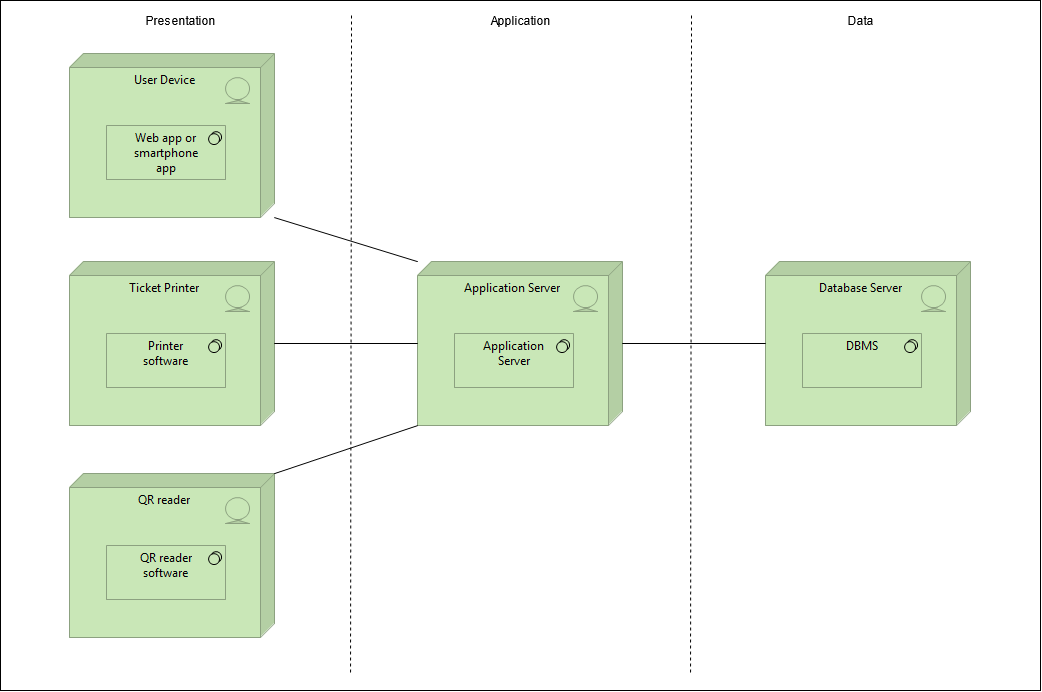
\includegraphics[scale=0.4]{Images/Archimate.png}\\
Customers line up at a store trough the web app or the smartphone application and their requests are sent to the 
\newpage
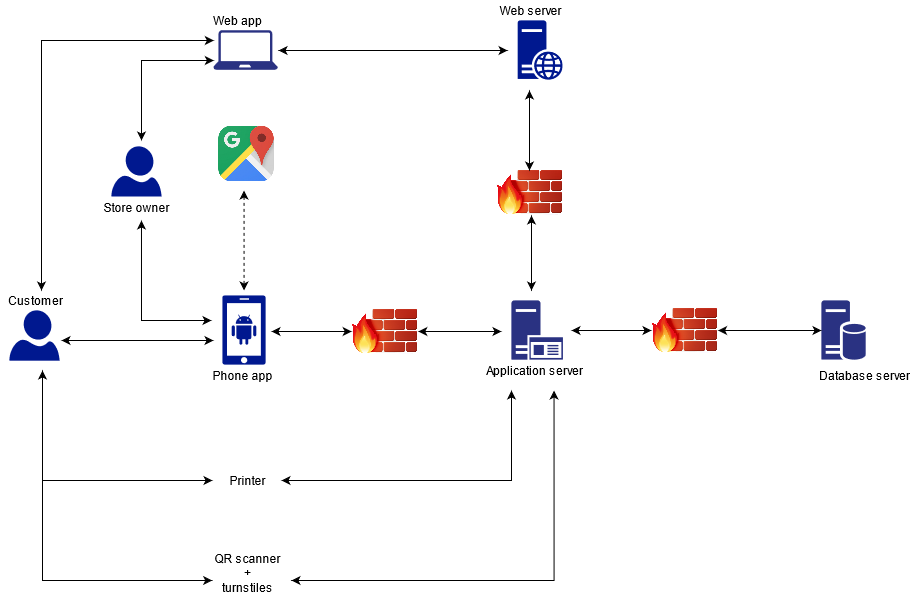
\includegraphics[scale=0.5]{Images/System Architecture.png}\\
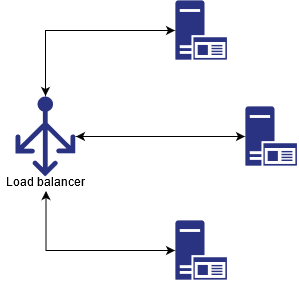
\includegraphics[scale=0.5]{Images/LoadBalancer.png}\\

\subsection{Component View}
Here we display the main component architecture of our S2B. Since the ApplicationServer contains all the business logic, we will describe in detail the structure of its subcomponents.
\begin{flushleft}
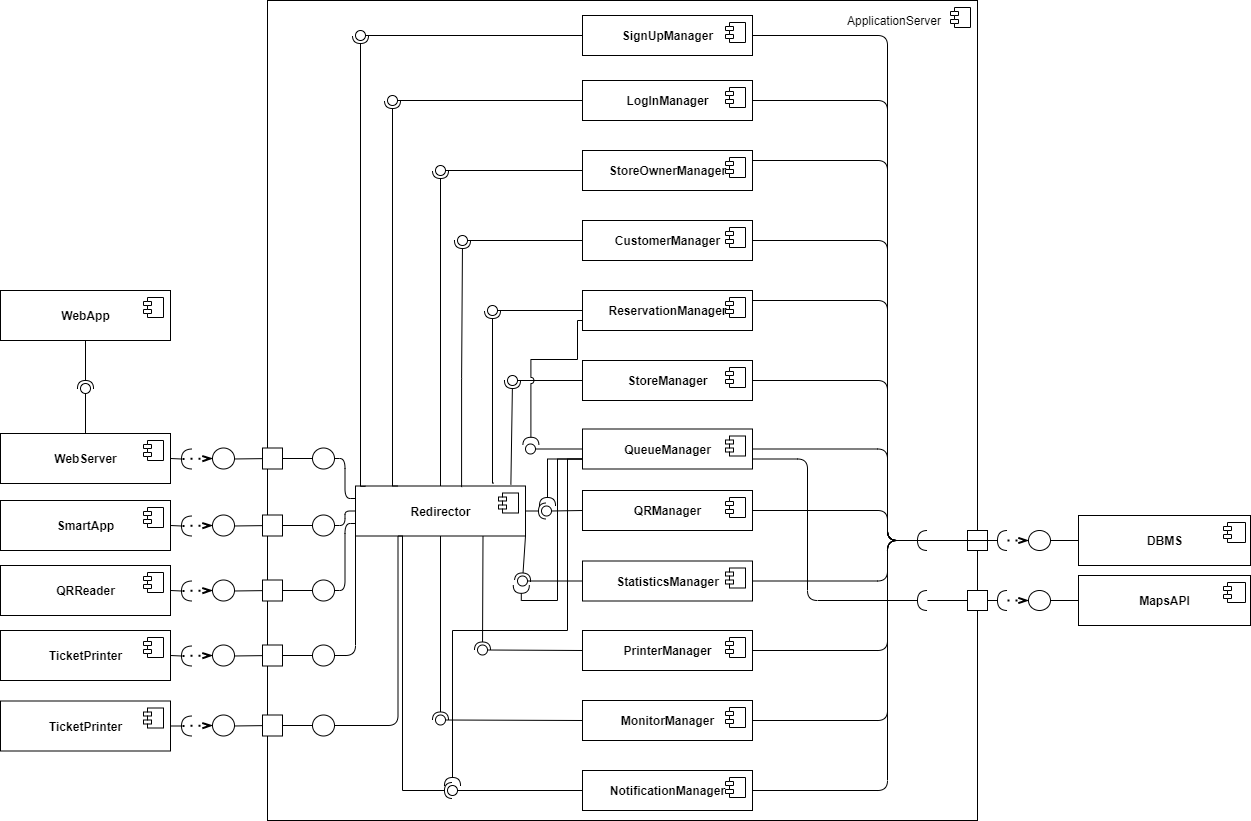
\includegraphics[scale=0.4]{Images/Component.png}
\end{flushleft}
\subsubsection{WebApp}
This component allows customer and store owners to access their respective services on a computer. It requires a WebServer.
\subsubsection{WebServer}
This component communicates directly with the ApplicationServer and serves web pages to implement the WebApp component.
\subsubsection{SmartApp}
This component allows customers and store owners to access their respective services on a smartphone, by interfacing with the ApplicationServer.
\subsubsection{QRReader}
This component reads user provided QRCodes and sends them to the ApplicationServer, thus enabling authentication for turnstiles.
\subsubsection{TicketPrinter}
This component accepts a user document and after having validated it through the ApplicationServer, it prints a reservation ticket with a QR.
\subsubsection{StoreMonitor}
This component updates periodically calling the ApplicationServer, which provides it with the number of the last authorized reservation, thus notifying customers in front of the store when they can enter.
\subsubsection{Redirector}
This component provides an external interface for the previously described components, and allows them to communicate with the components that are located within the ApplicationServer, that we describe below.
\subsubsection{SignupManager}
This component allows customers and store owners that provide a valid identification document to register to the service, thus gaining access to its functionalities, provided that they log in. It is called through WebApp or SmartApp, and needs to access the DBMS to search for existing users with same identification document (to avoid duplication), and to create a new user.
\subsubsection{LoginManager}
This component allows customers and store owners to log in the service, thus gaining access to its functionalities. It is called by WebApp and SmartApp components, and needs to access the DBMS to verify user credentials against the stored ones.
\subsubsection{StoreOwnerManager}
This component is accessed through WebApp or SmartApp and allows store owners to edit their credentials (obtained during sign up process), thus it needs access to DBMS.
\subsubsection{CustomerManager}
This component is accessed through WebApp or SmartApp and allows customers to edit their credentials (obtained during sign up process), thus it needs access to DBMS.
\subsubsection{ReservationManager}
This component is accessed through WebApp or SmartApp and allows customers to send a reservation for a specific store, to delete an existing reservation, or to view status of non expired reservations (QR code, position in queue, status) by accessing QueueManager. It needs to access DBMS to retireve the list of the departments of the store that the reservation targets and, in case of an immediate reservation, to verify that the store is open at the current time. It needs access to DBMS also to fetch the list of non expired user reservation along with their information, and to delete them if required.
\subsubsection{StoreManager}
This component is accessed through WebApp or SmartApp, and allows store owners to view owned stores, add new stores, delete existing stores or update information of existing stores, such as the list of departments and their respective maximum occupation. It needs to access the DBMS to execute the previous functions.
\subsubsection{QueueManager}
This component is accessed by the ReservationManager to add or remove a reservation from a queue of a specific store; whenever a reservation is added, this component accesses QRManager to generate an appropriate QR code for the reservation. It needs access to DBMS to get access to the current status of the queue of each store. It checks periodically the number of customers currently present, their location and the maximum occupation for every store and computes an estimated time that customers have to wait before gaining authorization to enter a specific store if such store has already reached maximum occupation. It checks periodically through MapsAPI an estimate of the time the customer needs to reach the store with his selected means of transport. If such time becomes lesser or equal to the time he/she needs to wait before entering the store, a notification is sent to the customer through NotificationManager if he/she uses a mobile application. This component accesses StatisticsManager to improve the computation of the time a customer needs to wait before being authorized to enter the store.
\subsubsection{QRManager}
This component is accessed by the QueueManager during the insertion of a reservation in the queue to produce the QR that will be used to identify the customer that created such reservation. It needs access to the DBMS: when QRReader reads a QR code, it accesses this component to retrieve from the data base the reservation (if any) to which this QR corresponds, and opens turnstiles depending on the state of the reservation.
\subsubsection{StatisticsManager}
This component is accessed by QueueManager to improve the estimate of the time that a customer needs to wait before being authorized to enter a specific store. This component is accessed by a store owner through WebApp or SmartApp to visualize statistics. This component accesses the DBMS periodically to obtain the data with which to generate the statistics, and to save such statistics.
\subsubsection{PrinterManager}
This component allows the store owner with WebApp or SmartApp to register a TicketPrinter. This component also allows customer identification through TicketPrinter by validating a provided identification document. This component needs to access the DBMS to register or unregister instances of TicketPrinter.
\subsubsection{MonitorManager}
This component allows to update periodically a StoreMonitor. It retrieves from the DBMS the number of the last authorized reservation.
\subsubsection{NotificationManager}
This component is accessed by the SmartApp to retrieve notifications. This component is sent notifications by the queue manager, whenever the time to reach the store becomes greater or equal to the estimate of the time to wait before being authoruzed to enter the store. This component saves unsent notifications in DBMS until it is able to dispatch them.